%%% 
%% Project Management 
%%% 
\chapter{Project Management}
\label{cha:project_management}

The management of projects has evolved to become more complex and diverse as
technology grows. One common characteristic shared by all projects is the
projection of activities and ideas. The management of a project allows the
explicit control of resources and budget as well as a coordinated path for a
successful project \citep{projMan86}.

This chapter consists of the management resources that were deployed within the
project. The chapter includes the initial plans developed for the project as
well as the accurate and concise plans of the project which were changed on a
constant basis to apprehend the need of the clients, the users, and the
development team of the project. Further more the psychology of the development
is briefly discussed to illustrate the change in the life cycle of the project.

% Project Overview 
\newpage 
%%%
%% Project Management :: Project Overview
%%%
\section{Project Overview}
\label{sec:project_overview}

The project began on Monday, 30$^t$$^h$ September 2013 and ended on Friday,
9$^t$$^h$ May 2014 allowing the team 32 weeks in order to plan, develop and
deploy the project as well as allowing sufficient time to produce the academic
and technical reports to accompany the product.

The planning of the project has been produced to incorporate all the academic
and technical deliverables. The major academic deliverables are:

\begin{itemize}
  \item Project Proposal
  \item Presentation of mid-point progress
  \item Submission of reports
  \item Final product demonstration
\end{itemize}

and the project milestone deliverables are:

\begin{itemize}
  \item Scope
  \item Software Requirements
  \item Design
  \item Development
  \item Testing
  \item Documentation
  \item Deployment
\end{itemize}

The following sections within this chapter show the progress of the project
where each of the deliverables were met accompanied by their predicted
completion dates to the actual dates when they were completed. There have been a
number of factors that have impacted the plans and these will be discussed in
the following sections.


% Planning 
\newpage 
%%%
%% Project Management :: Planning
%%%
\section{Planning}
\label{sec:planning}

% People Invloved 
\newpage 
%%%
%% Project Management :: People Involved
%%%
\section{People Involved}
\label{sec:people_involved}

A number of project stakeholders have already been outlined with the initial
problem analysis. Within this section the stakeholders that are involved with
the project will be redefined upon a more formal basis.

The `group' will be actively referred to throughout the project, and therefore 
the group will be defined. The group will have four members throughout the 
project, and these members are:

\begin{itemize}
  \item Leanne Butcher
  \item Luke Hackett
  \item Stuart Leader
  \item Mohammad Rahman
\end{itemize}

The project group is based largely upon democratic discussions and decisions,
however to ensure that group deadlocks do not occur Mohammad has been selected 
as the group leader.

The group will be assigned a project supervisor directly from the University.
The project supervisor will help to deal with an technical and non-technical
queries, whilst also ensuring the group remains upon a general focus. The
project supervisor may also suggest features and improvements to work that the
group managed to produce. The group's project supervisor is Dr. Gary Allen.

A weekly meeting will take place between all group members and the project 
supervisor to discuss all aspects of the project. This includes (but is not 
limited to) project issues, software development issues, research findings, 
possible improvements and code reviews.

As the project is a formal assessment, the project assessor and moderator will 
be classified as indirect stakeholders within the project. Dr Sotirios Batsakis
and Dr Colin Venters have been assigned the roles of project assessor and 
project moderator respectfully. Both the project assessor and moderator will 
have a limited amount of contact time with the group, but will be present at 
formal presentations that are scheduled throughout the year.

The project formally does not have any clients associated with the work, however
Dr Hugh Osborne has offered to fill a client-like role within the project. Hugh
has a keen interest in cryptic crosswords and the problem area that the group
intends to sole. The role of the client for the group project will be to input
ideas and potential requirements which Hugh, as an experienced solver of cryptic
crosswords, would consider to be necessary.


% Ethics And Professionalism 
\newpage 
%%%
%% Project Management :: Ethics and Professionalism
%%%
\section{Ethics and Professionalism}
\label{sec:ethics_and_professionalism}

% Psychology of Software Development 
\newpage
%%%
%% Project Management :: Psycholoogy of Software Development
%%%
\section{Psycholoogy of Software Development}
\label{sec:psycholoogy_of_software_development}

% Estimation And Costing 
\newpage 
%%% 
%% Project Management :: Estimation and Costing 
%%% 
\section{Estimation and Costing} 
\label{sec:estimation_and_costing}

The costs of a software development project are primarily the costs of the effort involved. The three main areas which correspond to the cost of a software project include:

\begin{itemize}
	\item Hardware and software costs including maintenance
	\item Travel and training costs
	\item Effort costs (Costs of paying software engineers).
\end{itemize}

The main cost that will be discussed in this section is the effort costs as this is the most adequate cost that can be calculated for this project. In order to estimate the project costs the volume of the software must be calculated. This can be done by calculating number of Source lines of Code(SLOC) also calculated as Thousands of lines of Code (KLOC). The most common estimating metric is the Constructive Cost Model (COCOMO) and the new COCOMO II. Function points is another metrics that can be used to estimate the project. 

COCOMO was originally devloped by \citet{see81}. It has since been re-developed as COCOMO II \citep{cocomo2}. 

The basic COCOMO formula is:

Effort Applied (Person Months)
\[
	E=a(KLOC)^{b}
\]

Development Time(Months)
\[
	DT=cE^{d}
\]

People Required
\[
	P=E/D
\]

\begin{table}[H]
  	\centering
  	\small
    \begin{tabular}{|l|l|l|l|l|}
    \hline
    Mode          & a   & b    & c   & d    \\ \hline
    Organic       & 2.4 & 1.05 & 2.5 & 0.38 \\ \hline
    Semi Detached & 3.0 & 1.12 & 2.5 & 0.35 \\ \hline
    Embeded       & 3.6 & 1.20 & 2.5 & 0.32 \\ \hline
    \end{tabular}
    \caption {Basic COCOMO}
\end{table}

The cryptic solver best suits the Organic mode because the team is small consisting of four members who have experience working with requirements. On this basis and the time constraint factors the project can be estimated. The development time allocated for the project is 3.25 months which is the 98 days calculated from the project plan. This has been considered to exclude time for other academic deliverables and to mainly focus upon the actual development. There fore according to \citet{cocomo2} the project can be estimated as followed:

Effort Applied (Person Months)
\[
	E=2.4(5)^{1.05} = 13
\]
Development Time (Months)
\[
	DT=2.5(13)^{0.38} = 6.5 
\]
People Required
\[
	P=13/6.5 = 2
\]

Now to evaluate this against the number of actual team members we can do the following.

Development Time (Months)
\[
	DT=2.5(13)^{0.38}/2 = 3.25
\]
People Required
\[
	P=13/3.25 = 4
\]


The estimated number of lines of code SLOC is therefore 5(thousand). Upon completion of the project the COCOMO model was applied to see how closely the original estimation was made. In total there are 5721 SLOC and therefore applying the same algorithms as before produced the following results.

Effort Applied (Person Months)
\[
	E=2.4(6)^{1.05} = 15
\]
Development Time (Months)
\[
	DT=2.5(13)^{0.38}/2 = 3.5
\]
People Required
\[
	P=15/3.5 = 4
\]






% Allocation Of Work 
\newpage 
%%% 
%% Project Management :: Allocation of Work 
%%% 
\section{Allocation of Work}
\label{sec:allocation_of_work}

The allocation of work was primarily voluntary from members of the team. During the first term the tasks were delegated by all team members to each other clarifying on the different components that they would be working on in order to ensure there was no clash between each other. The dates for work to be completed was set by the team leader to ensure that the team was working on schedule. Tasks were delegated on a weekly basis at the group meetings. The minutes can be found in the appendix. 

Activities were split into a series of stages:

\begin{itemize}
    \item Familiarization
    \item Planning and preparation
    \item Implementation
    \item Completion
\end{itemize}

During the familiarization stage the individual members of the group got to know each other very quickly because the members have been studying on the same course over the period of 2009 to 2013 although this is the first time that all members worked together on a single project. The group initially took the time to identify areas of interest and the skills they have, which brought a sense of the strengths and weaknesses of the group.

For the planning and preparation stage the initial plans were drawn up by the group and each member stated what they thought is required to be done. Elements of the initial tasks were agreed by team members and the project supervisor. The main planning from here forward was managed by the team leader and agreed upon by the team members. Effective communication was addressed through the use of the Social Media website Facebook although more formal tools were used such as email and OneDrive(SkyDrive). During implementation the use of a version control system (GitHub) enabled the team to manage workloads effectively and track remaining issues that coincide with the project plan. The total number of issues raised was 66 although not all issues according to the project plan were raised as they were done earlier then planned. Figures \ref{fig:issues1} to \ref{fig:issues2} show all the closed issues at the end of the project.

\begin{figure}[H]
  \centering
  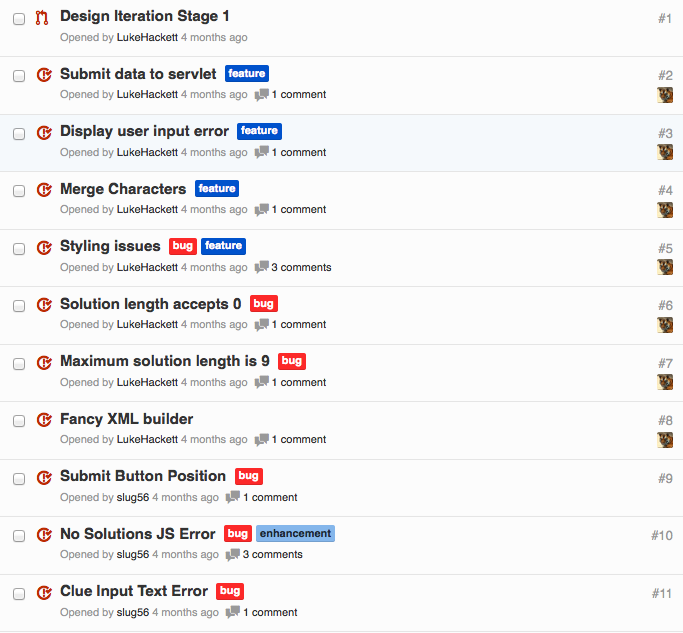
\includegraphics[width=\linewidth]{images/issues1.png}
  \caption{Issues 1}
  \label{fig:issues1}
\end{figure}
\begin{figure}[H]
  \centering
  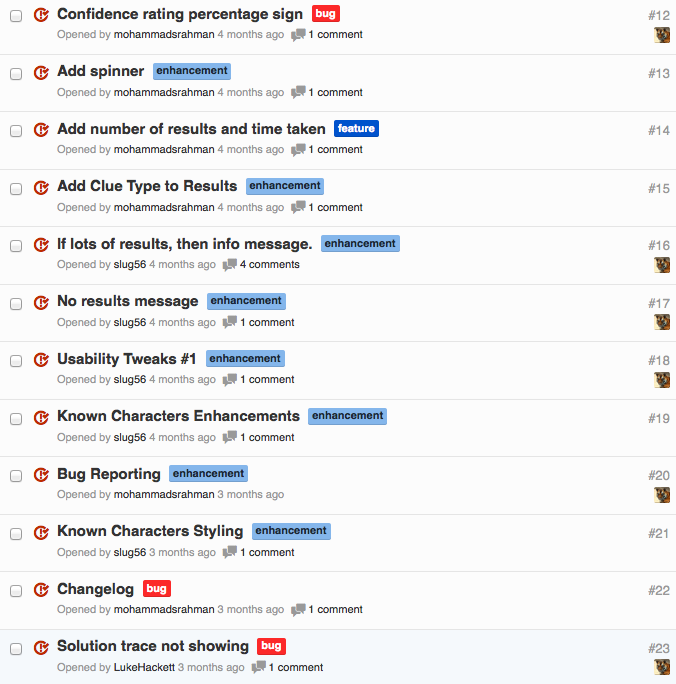
\includegraphics[width=\linewidth]{images/issues2.png}
  \caption{Issues 2}
  \label{fig:issues2}
\end{figure}
\begin{figure}[H]
  \centering
  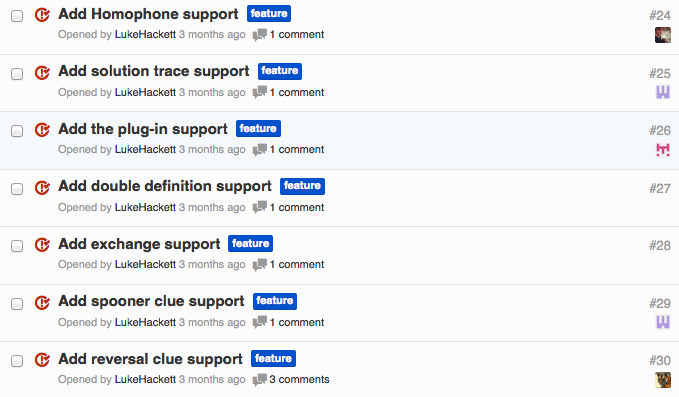
\includegraphics[width=\linewidth]{images/issues3.png}
  \caption{Issues 3}
  \label{fig:issues3}
\end{figure}
\begin{figure}[H]
  \centering
  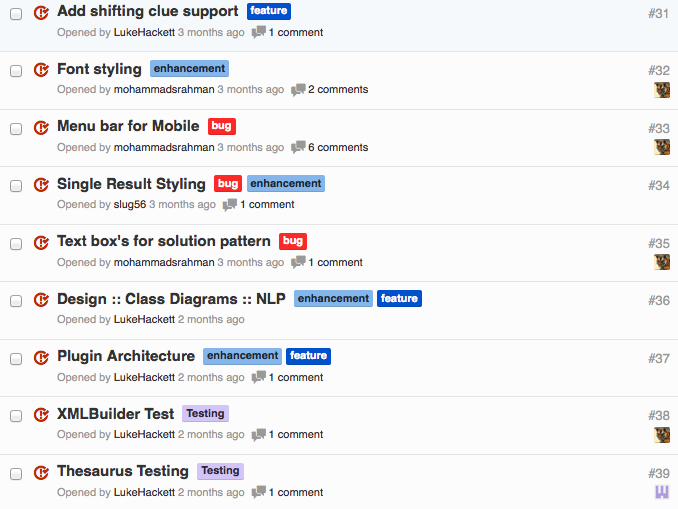
\includegraphics[width=\linewidth]{images/issues4.png}
  \caption{Issues 4}
  \label{fig:issues4}
\end{figure}
\begin{figure}[H]
  \centering
  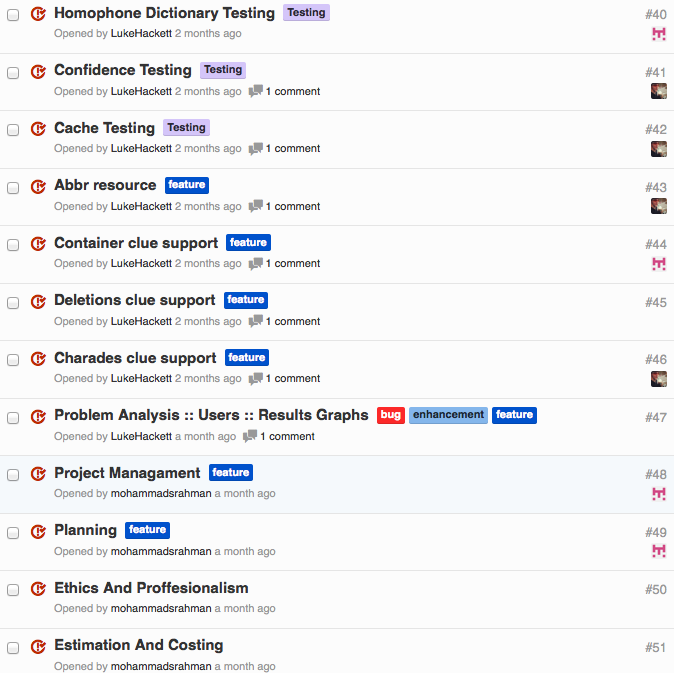
\includegraphics[width=\linewidth]{images/issues5.png}
  \caption{Issues 5}
  \label{fig:issues5}
\end{figure}
\begin{figure}[H]
  \centering
  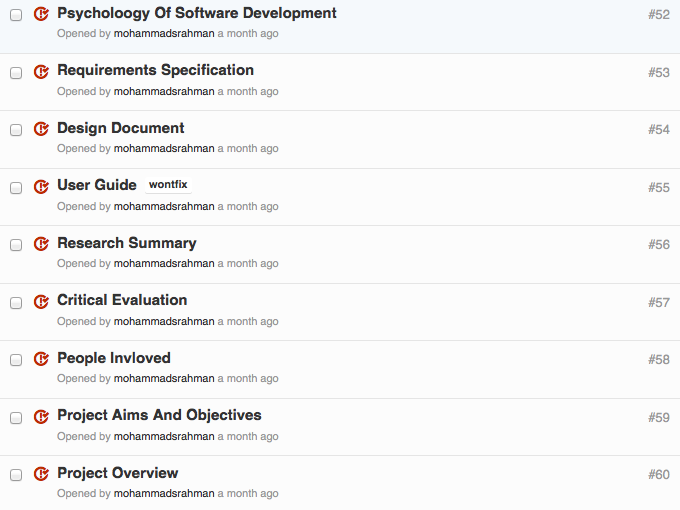
\includegraphics[width=\linewidth]{images/issues6.png}
  \caption{Issues 6}
  \label{fig:issues6}
\end{figure}
\begin{figure}[H]
  \centering
  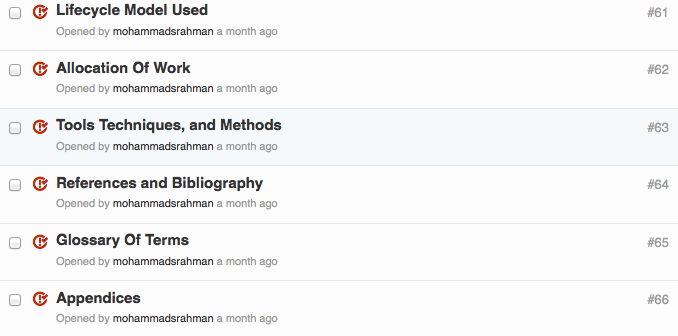
\includegraphics[width=\linewidth]{images/issues7.png}
  \caption{Issues 7}
  \label{fig:issues7}
\end{figure}

The tasks in the first term mainly focused upon individuals to be issued the task and produce the work by the following week and to be reviewed by the rest of the team members in the meetings. By the second term when development started the tasks were delegated to be worked in pairs. The architecture of the system was primarily developed by Stuart Leader and interfaces by Luke Hackett but in collaboration with the remainder of the team members. After the architecture of the system had been produced each team member selected a task such as a solver and attempted to write the algorithms. For the low level clues an individual was able to produce the algorithms but for the further solvers the team had to collaborate and work together.

Finally during the documentation and report writing most of the report was produced in parallel to term one and the research. Returning to the report after development proved to be beneficial as team members were once again able to select components which required to be done and produce the work. Each produced work has been throughly checked over by the other team members to ensure that anything that has been produced and written is up to its standards.

% Lifecycle Model Used 
%\newpage 
%\input{lifecycle_model_used}

% Tools Techniques and Methods 
%\newpage 
%\input{tools_techniques_and_methods}
